\chapter{The Epsilon Generation Language (EGL)}
\label{sec:EGL}

EGL provides a language for M2T in the large.   EGL is a model-driven
template-based code generator, built atop Epsilon, and re-using all
of EOL. In this section, we discuss the  design of EGL and its
construction from existing Epsilon tools.

\section{Abstract Syntax}
Figure \ref{fig:abstractsyntax} depicts the abstract syntax of EGL's core functionality.

\begin{figure}[htbp]
  \begin{center}
    \leavevmode
    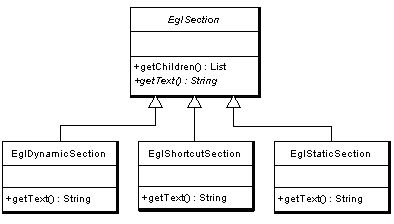
\includegraphics[scale=0.80]{images/EglAbstractSyntax.png}
  \end{center}
  \caption{The abstract syntax of EGL's core.}
  \label{fig:abstractsyntax}
\end{figure}

In common with other template-based code generators, EGL defines
\emph{sections}, from which templates may be constructed. Static
sections delimit sections whose contents appear verbatim in the
generated text. Dynamic sections contain executable code that can be
used to control the generated text.

In its dynamic sections, EGL re-uses EOL's mechanisms for structuring
program control flow, performing model inspection and navigation, and
defining custom operations.  EGL provides an EOL object, \verb|out|,
for use within dynamic sections.  This can be used to perform
operations on the generated text, such as appending and removing
strings and specifying the type of text to be generated.

EGL also provides syntax for defining \textit{dynamic output}
sections, which provide a convenient shorthand for outputting text
from within dynamic sections. Similar syntax is often provided by
template-based code generators.

\section{Concrete Syntax}
\label{concretesyntax}

The concrete syntax of EGL mirrors the style of other
template-based code generation languages. The tag pair \verb|[% %]| is
used to delimit a dynamic section. Any text not enclosed in such a tag
pair is contained in a static section. Listing
\ref{lst:basic} illustrates the use of dynamic and static sections to
form a basic EGL template.

\begin{lstlisting}[basicstyle=\ttfamily\footnotesize, tabsize=2, flexiblecolumns=true, caption=A basic EGL template., label=lst:basic]
[% for (i in Sequence{1..5}) { %]
i is [%=i%]
[% } %]
\end{lstlisting}

The \emph{[\%=expr\%]} construct is shorthand for \emph{[\%
  out.print(expr); \%]}, which appends \emph{expr} to the output
generated by the transformation. Note that the \verb|out| keyword also
provides \emph{println(Object)} and \emph{chop(Integer)} methods, which
can be used to construct text with linefeeds, and to remove the
specified number of characters from the end of the generated text.

EGL exploits EOL's model querying capabilities to output text from
models specified as input to transformations. For example, the EGL
template depicted in Listing \ref{lst:oo} may be used to generate text
from a model that conforms to a metamodel that describes an
object-oriented system.

\begin{lstlisting}[basicstyle=\ttfamily\footnotesize, tabsize=2, flexiblecolumns=true, caption=Generating the name of each Class contained in an input model., label=lst:oo]
[% for (class in Class.allInstances) { %]
[%=class.name%]
[% } %]
\end{lstlisting}

\section{Parsing and Preprocessing}
EGL provides a parser which generates an abstract syntax tree comprising static, dynamic and dynamic output nodes for a given template. A preprocessor then translates each section into corresponding EOL: static and dynamic output sections generate \verb|out.print()| statements. Dynamic sections are already specified in EOL, and require no translation.

Consider the EGL depicted in Listing \ref{lst:basic}.  The
preprocessor produces the EOL
shown in Listing
\ref{lst:preprocessor-eol} -- the \verb|[% %]| and \verb|[%=  %]| tag pairs have been removed, and the text to be output is translated into \verb|out.print()| statements.

\begin{lstlisting}[basicstyle=\ttfamily\footnotesize, tabsize=2, flexiblecolumns=true, caption=Resulting EOL generated by the preprocessor., label=lst:preprocessor-eol]
for (i in Sequence{1..5}) {
   out.print(`i is ');
   out.print(i);
   out.print(`\r\n');
}
\end{lstlisting}

When comparing Listings \ref{lst:basic} and \ref{lst:preprocessor-eol}, it can be seen that the template-based syntax is more concise, while the preprocessed syntax is arguably more readable. For templates where there is more dynamic than static text, such as the one depicted in Listing \ref{lst:basic}, a template-based syntax is often less readable. However, this loss of readability is somewhat mitigated by EGL's developer tools, which are discussed in Section \ref{Tool Support}. By contrast, for templates that exhibit more static than dynamic text, a template-based syntax is often more readable than its preprocessed equivalent.

\section{Deriving EGL from EOL}

In designing functionality specific to M2T transformation, one option
was to 
enrich the existing EOL syntax with  keywords such as \emph{print}, \emph{contentType} 
and \emph{merge}.  However, EOL underpins all Epsilon
languages, and the additional keywords were needed only for M2T.
Furthermore, the refactorings needed to support the new keywords
affect many components -- the lexer, parser, execution context and
execution engine -- complicating maintenance and use by other developers.
Instead, we define a minimal syntax for EGL, allowing easy
implementation of an EGL execution engine as a simple preprocessor for EOL. 
 

The EGL execution engine augments the default context used by EOL
during execution with two read-only, global variables: \emph{out}
(Section \ref{concretesyntax}) and \emph{TemplateFactory} (Section
\ref{Co-ordination}). The \emph{out} object defines methods for
performing operations specific to M2T translation, and the
\emph{TemplateFactory} object provides methods for loading other
templates. The implementation for the latter was extended, late in the
EGL development, to provide support for accessing templates from a
file-system -- a trivial extension that caused no migration problems
for existing EGL templates, due to the way in which EGL extends EOL.

\section{Co-ordination}
\label{Co-ordination}
In the large, M2T transformations need to be able to not only generate
text, but also files, which are then used downstream as development
artefacts.  An M2T tool must provide the language constructs for
producing files and manipulating the local file system.  Often, this
requires that the destination, as well as the contents, be dynamically
defined at a transformation's execution time.

The EGL co-ordination engine supplies mechanisms for generating text
directly to files.  The design encourages decoupling of generated text
from output destinations. The \emph{Template} data-type is provided to
allow nested execution of M2T transformations, and operations on
instances of this data-type facilitate the generation of text directly
to file. A factory object, \emph{TemplateFactory}, is provided to
simplify the creation of \emph{Template} objects.  In Listing
\ref{lst:co-ordination}, these objects are used in an EGL template
that loads the the EGL template in Listing \ref{lst:oo} from the file,
ClassNames.egl, and writes out to disk the text generated by executing
ClassNames.egl.

\begin{lstlisting}[basicstyle=\ttfamily\footnotesize, tabsize=2, flexiblecolumns=true, caption=Storing the name of each Class to disk., label=lst:co-ordination]
[%
  var t : Template := TemplateFactory.load(`ClassNames.egl');
  t.process();
  t.store(`Output.txt');
%]
\end{lstlisting}

This approach to co-ordination allows EGL to be used to generate one
or more files from a single input model. Moreover, EGL's co-ordination
engine facilitates the specification of platform-specific details (the
destination of any files being generated) separately from the
platform-independent details (the contents of any files being
generated).

\section{Merge Engine}
EGL provides language constructs that allow M2T transformations to
designate regions of generated text as \textit{protected}. The
contents of protected regions are preserved every time a M2T
transformation generates text to the same destination.

Protected regions are specified by the \emph{preserve(String, String,
  String, Boolean, String)} method on the \verb|out| keyword. The first two parameters define the comment delimiters
of the target language. The other parameters provide the name,
enable-state and content of the protected region, as
illustrated in Listing \ref{lst:preserve}.

\begin{lstlisting}[basicstyle=\ttfamily\footnotesize, tabsize=2, flexiblecolumns=true, caption=Protected region declaration using the preserve method., label=lst:preserve]
[%=out.preserve(`/*', `*/', `anId', true,
                `System.out.println(foo);')
%]
\end{lstlisting}

A protected region declaration may have many lines, and use many EGL
variables in the contents definition.  To enhance readability, EGL
provides two additional methods on the \verb|out| keyword:
\emph{startPreserve(String, String, String, Boolean)} and
\verb|stopPreserve|.  Listing \ref{lst:startpreserve} uses these to
generate a protected region equivalent to that in Listing
\ref{lst:preserve}.

\begin{lstlisting}[basicstyle=\ttfamily\footnotesize, tabsize=2, flexiblecolumns=true, caption=Protected region declaration., label=lst:startpreserve]
[%=out.startPreserve(`/*', `*/', `anId', true)%]
System.out.println(foo);
[%=out.stopPreserve()%]
\end{lstlisting}

Because an EGL template may contain many protected regions, EGL also
provides a separate method to set the target language generated by the
current template, \emph{setContentType(String)}. By default, EGL recognises Java, HTML, Visual Basic,
Perl and EGL as valid content types. An alternative configuration file
can be used to specify further content
types. Following a call to \verb|setContentType|, the first two
arguments to the \verb|preserve| and \verb|startPreserve| methods can
be omitted, as shown in Listing \ref{lst:contenttype}.

\begin{lstlisting}[basicstyle=\ttfamily\footnotesize, tabsize=2, flexiblecolumns=true, caption=Setting the content type., label=lst:contenttype]
[% out.setContentType(`Java'); %]
[%=out.preserve(`anId', true, `System.out.println(foo);')%]
\end{lstlisting}

Because some languages define more than one style of comment
delimiter, EGL allows mixed use of  the styles for \verb|preserve| and
\verb|startPreserve| methods.

Once a content type has been specified, a protected region may be declared entirely from a static section, using the syntax  in Listing \ref{lst:manualpr}.

\begin{lstlisting}[basicstyle=\ttfamily\footnotesize, tabsize=2, flexiblecolumns=true, caption=Declaring a protected region from within a static section., label=lst:manualpr]
[% out.setContentType(`Java'); %]
// protected region anId [on|off] begin
System.out.println(foo);
// protected region anId end
\end{lstlisting}

When a template that defines one or more protected regions is
processed by the EGL execution engine, the target output destinations
are interrogated and existing contents of any protected regions are
preserved. If either the output generated by from the template or the
existing contents of the target output destination contains protected
regions, a merging process is invoked. Table \ref{tab:merging} shows
the default behaviour of EGL's merge engine.

\begin{table}[htbp]
  \begin{center}
  \begin{tabular}{|l|l|l|}
  \hline
  \multicolumn{2}{|l|}{\textbf{Protected Region Status}} & \multirow{2}{*}{\textbf{Contents taken from}} \\
  \textbf{Generated} & \textbf{Existing} & \\
  \hline
  On & On     & Existing  \\
  On & Off    & Generated \\
  On & Absent & Generated \\
  \hline
  Off & On     & Existing  \\
  Off & Off    & Generated \\
  Off & Absent & Generated \\
  \hline
  Absent & On  & Neither (causes a warning) \\
  Absent & Off & Neither (causes a warning) \\
  \hline
  \end{tabular}
  \end{center}
\caption{EGL's default merging behaviour.}
\label{tab:merging}
\end{table}

\section{Readability and traceability} 
Conscientious developers apply various \emph{conventions} to produce
readable code.  EGL encourages template developers to prioritise the
readability of templates over the text that they generate. EGL provides a number of text post-processors -- or
\textit{beautifiers} -- that can be executed on output of
transformations to improve readability.  Currently, beautifiers are
invoked via Epsilon's extensions to Apache Ant, an
XML-based build tool for Java.

EGL also provides a traceability API, as a debugging aid, and to
support auditing of the M2T transformation process.  This API
facilitates exploration of the templates executed, files affected and
protected regions processed during a transformation.  Figure
\ref{fig:traceability} shows sample output from the traceability API
after execution of an EGL M2T transformation to generate Java
code from an instance of an OO metamodel.

The beautification interface is minimal, in order to allow re-use of existing 
code formatting algorithms. Consequently, there is presently no traceability support 
for beautified text. However, due to the coarse-grained approach employed by 
EGL's traceability API, this has little impact: Clicking on a beautified protected 
region in the traceability view might not highlight the correct line in the editor.

\begin{figure}[htbp]
  \begin{center}
    \leavevmode
    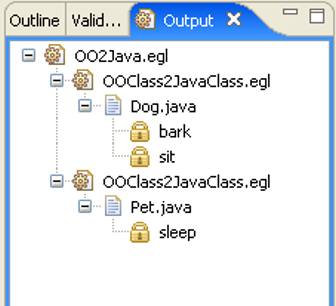
\includegraphics[scale=0.6]{images/TraceView}
  \end{center}
  \caption{Sample output from the traceability API.}
  \label{fig:traceability}
\end{figure}

\subsection{Tool Support}
\label{Tool Support}
The Epsilon platform provides development tools for the Eclipse
development environment. Re-use of Eclipse APIs allows
Epsilon's development tooling to incorporate a large number of
features with minimal effort. Furthermore, the flexibility of the
plug-in architecture of Eclipse enhances modular authoring of
development tools for Epsilon.

In addition to the traceability view shown in Figure
\ref{fig:traceability}, EGL includes an Eclipse editor and an outline
view. In order to aid template readability, these tools provide syntax 
highlighting and a structural overview for EGL templates, respectively. Through its 
integration in the Epsilon perspective, EGL provides an Eclipse workbench 
configuration that is tailored for use with Epsilon's development tools.

%\begin{figure}[htbp]
%  \begin{center}
%    \leavevmode
%    \includegraphics[scale=0.66]{EglWorkspace.png}
%  \end{center}
%  \caption{The EGL editor and outline view.}
%  \label{fig:editorandview}
%\end{figure}

EGL, like other Epsilon languages, provides an Apache ANT
task definition, to facilitate invocation of model-management activies
from within a build script.